\subsection{Sub Unit Power Supply}
\subsubsection{Block Diagram}
\createfigurewsvg{../Modular Design/Sub-Unit-PSU/Figures/sub-unit-psu.svg}{Sub Unit Power Supply Architectural Diagram}{fig:sub-unit-psu-bd}
\subsubsection{Schematic Diagram}
\begin{landscape}
  \begin{center}
  \begin{figure}[H]
    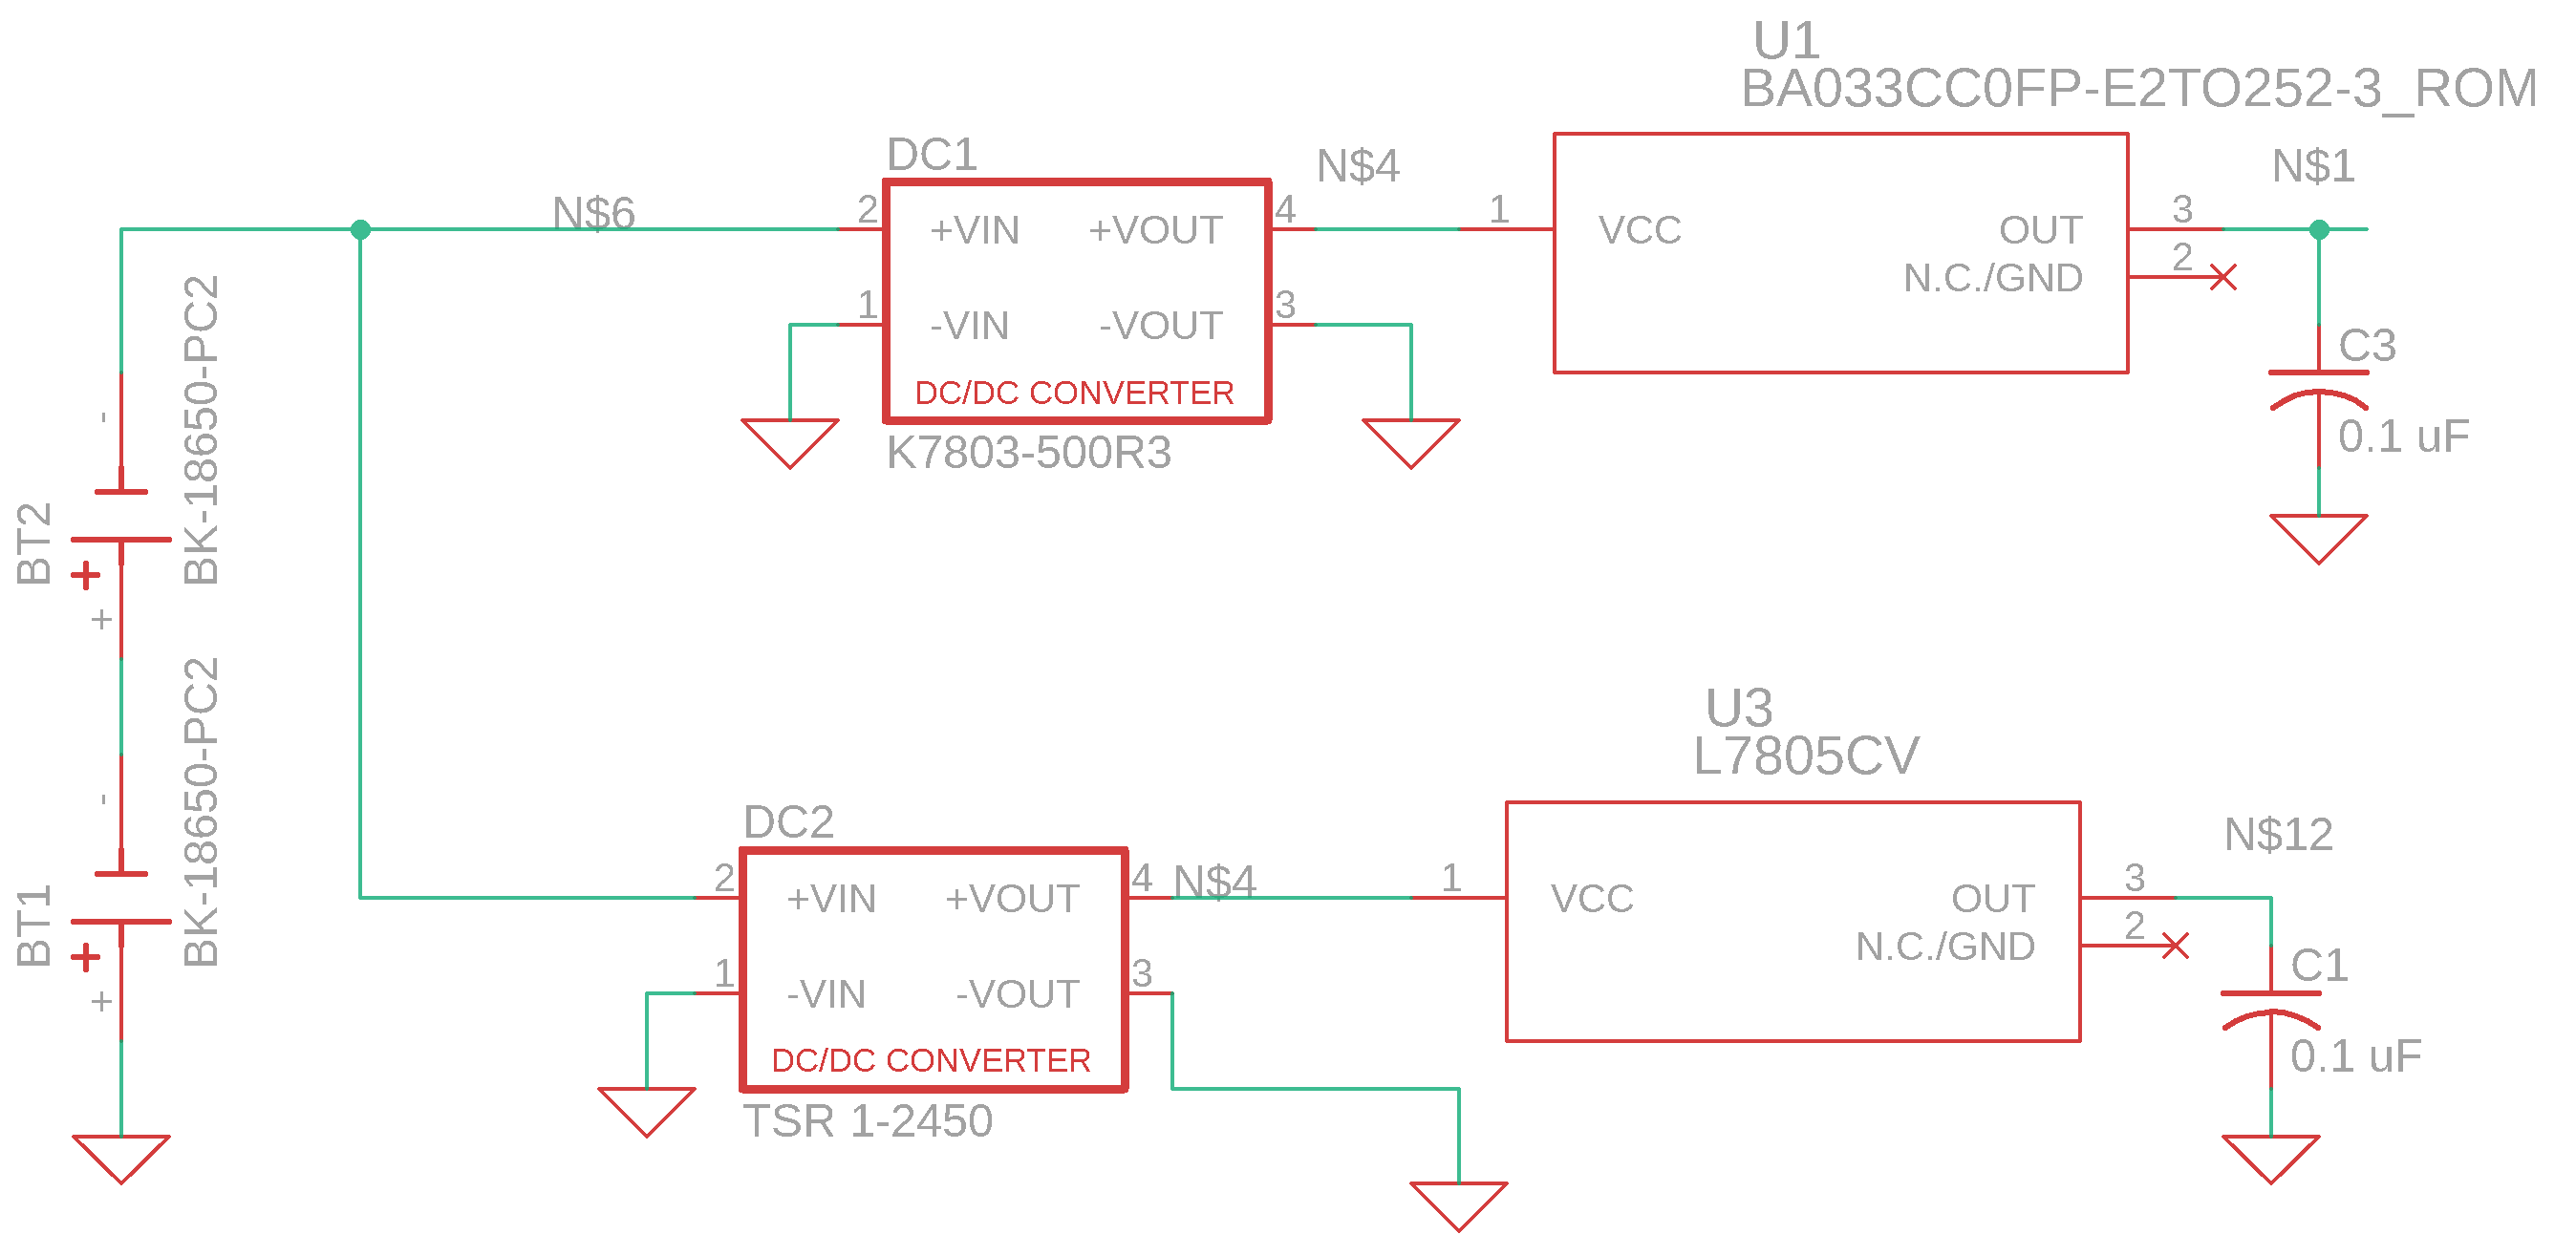
\includegraphics[width=1.6\textwidth, left]{../Modular Design/Sub-Unit-PSU/Figures/sub-unit-psu.png}
    \caption{Main Sub PSU Schematic}
    \label{fig:sub-psu-schematic}
  \end{figure}
  \end{center}
\end{landscape}
\subsubsection{Power Analysis, Loading, Driving, and Compatibility}
The sub unit PSU operates in a very similar fashion to the main unit PSU when mains power is not available. BT1 and BT2 supply a 3.3\si{\V} (K7803-500R3) \cite{K7803500R3} and a 5\si{\V} (TSR 1-2450) \cite{TSR12450} DC/DC converter in parallel. As analyzed in the main unit PSU, both DC/DC converters require less than 6.5\si{\V} to conduct properly and since the battery is directly supplying the DC/DC converters, they will receive a nominal voltage of 7.2\si{\V} since BT1 and B2 are 3.6\si{\V} cells in series.\\ U1 (BA33BC0T) \cite{BA33BC0T} U2 (BA33BC0T) will also be compatible as analyzed above since their maximum input are above 3.3\si{\V} and 5\si{\V} respectively. As for C1 and C3, they have a voltage rating of 50\si{\V}, therefore are compatible being in parallel with the outputs of U1 and U2.
\subsubsection{Reliability \& Design Criteria}
The sub unit power supply only has to regulate the battery voltage to 3.3\si{\V} and 4\si{\V} for the MCU and Bluetooth module respectively at a high efficiency in order to achieve a 2 year life time of the design.
\subsubsection{Level of Completion}
\begin{table}[!ht]
  \begin{tabularx}{\textwidth}{|X|X|}
    \hline
    \multicolumn{2}{|X|}{Sub Unit PSU}\\
    \hline
    Integration&\begin{itemize}
                  \item 4\si{\V} Power Rail
                  \item 3.3\si{\V} Power Rail
                \end{itemize}\\
    \hline
  \end{tabularx}
\end{table}
